\documentclass[11pt,a4paper]{article}
\usepackage[utf8]{inputenc}
\usepackage[english]{babel}
\usepackage{amsmath}
\usepackage{amsfonts}
\usepackage{amssymb}
\usepackage{mathrsfs}
\usepackage{gensymb}
\usepackage{fancyhdr}
\usepackage[left=1.5cm,right=1.5cm,top=2.5cm,bottom=2cm]{geometry}
\usepackage{adjustbox}
\usepackage{booktabs}  
\usepackage{threeparttable} 
\usepackage{makecell}
\usepackage{parskip}
\usepackage{graphicx}
\usepackage{listings}


\begin{document}
\title{MCMC Sampling Methods}
\pagestyle{fancy}

{
\fancyhf{}
\rhead{11 June 2018}
\lhead{Yunzhe Li, Yizi Zhang, Ruriko Imai} 
\cfoot{\thepage}
}

\vspace*{\fill}
\begin{center}
\subsection*{ 
\huge Comparing Metropolis and Gibbs Sampling Method
}
\end{center}

\begin{center}
Yunzhe Li: madli@ucdavis.edu \\
Ruriko Imai: raimai@ucdavis.edu \\
Yizi Zhang: yizzhang@ucdavis.edu
\end{center}
\bigskip
\bigskip
\bigskip
\bigskip
\bigskip
\bigskip
\bigskip
\bigskip
\bigskip
\bigskip
\bigskip
\bigskip


\begin{center}
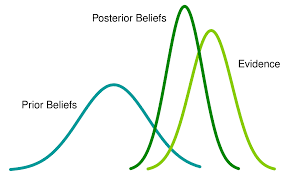
\includegraphics[scale=1.5]{images/cover.png}
\end{center}
\vspace*{\fill}
\newpage

% =================== Introduction =============================

\section*{Introduction}
The purpose of this project is to explore sampling methods derived from algorithms in the Monte Carlo Markov Chain (MCMC) family called the Metropolis sampling and Gibbs sampling methods. These MCMC algorithms are used in a bayesian setting where direct sampling from the posterior distribution is difficult. By sampling from the posterior we will be able to estimate mean and other parameters to further analyze the data. In order to check for performance, speed and accuracy of those sampling methods, we shall use a known posterior distribution so the distribution obtained from Metropolis and Gibbs sampling methods can be compared. Therefore, the  setting of the sampling distribution is Multinomial - Dirichlet conjugate with K = 3 categories with two-dimensional parameters to update. 

% =================== Difference ===============================

\section*{Difference between Gibbs and Metropolis Algorithm}
Metropolis-Hastings sampler is the umbrella algorithm for both Gibbs and Metropolis sampling methods. These sampling methods are used when direct sampling is deemed difficult to perform on a given posterior distribution. Gibbs sampling is a special case of Metropolis hastings algorithm with a probability acceptance rate of 1. Metropolis sampling is also a special case of Metropolis hastings, requiring a symmetric proposal distribution. Although the algorithms are slightly different, the purpose is to sample from the posterior distribution. 
\newline
Some issues to consider are: 
 
\begin{itemize}
 \item determine a good burn-in amount to decrease dependence on starting values  
 \item determine a good thinning amount to decrease autocorrelation
 \item determine a good proposal distribution for Metropolis sampler
 \item partial correlation between parameters
 \item convergence diagnostics
\end{itemize}
 
We will explore these issues throughout this simulation process.	

% ==================== Set-Up ===================================

\section*{Set-Up}
\begin{itemize}
	\item Data: 
	\begin{itemize}
		\item True parameters: $\theta_{1} = 0.1$, $\theta_{2} = 0.7$, $\theta_{3} = 0.2$
		\item Hyperparameters: $\alpha_{1} = 2$, $\alpha_{2} = 2$, $\alpha_{3} = 2$ 
	\end{itemize}
	\item Prior: $X_{i} | \theta \overset{iid}{\sim} Multinom(n, \theta_{1}, \theta_{2}, \theta_{3}); i = 1, \dots, n$
	\item Likelihood function: (singular) $Multinom(\theta_{1},\theta_{2},\theta_{3})$.
	\item Proposal: $Dirichlet(\alpha_{1}, \alpha_{2}, \alpha_{3})$
	\item Posterior: $Dirichlet(\alpha_{1}+\sum{X_{1i}}, \ \alpha_{2}+\sum{X_{2i}} + \alpha_{3}+\sum{X_{3i}})$
\end{itemize}

\newpage

% ==================== Algorithm =================================

% \section*{Algorithms}
% Metropolis algorithm: 
% \begin{itemize}
% \item Choose a starting point for $\theta$'s from a starting distribution
% \item For t = 1, 2, $\dots$
% 	\begin{itemize}
% 		\item Sample a proposed $\theta^{\star}$ from a symmetric jumping/proposal distribution at time t. 
% 		\item Calculate the density ratio: \\
% 		\begin{equation}
% 			ratio = \frac{p(\theta^{\star})|y}{\theta^{t-1}|y}
% 		\end{equation}
% 		\item   Set:\begin{equation}
%     				\theta^t=
%     				\begin{cases}
%              		\theta^{\star}, & \text{with propability min(ratio, 1)} \\
%    		 	  		\theta^{t-1}, & \text{otherwise}
%    		 			\end{cases}
%   			    \end{equation}

% 	\end{itemize}
% \end{itemize}
% Gibbs algorithm:
% \begin{itemize}
% 	\item Set initial values for $\theta$'s
% 	\item Set $Y = \frac{\theta_{1}}{1-\theta_{2}}|\theta_{2}$\\
% 	\ \ \ $Y \sim Beta(\alpha_{1}+\sum{X_{1i}}, \ \alpha_{2}+\sum{X_{2i}} + \alpha_{3}+\sum{X_{3i}})$
% 	\item Set $Z = \frac{\theta_{2}}{1-\theta_{1}}|\theta_{1}$\\
% 	\ \ \ $Z \sim Beta(\alpha_{2}+\sum{X_{2i}}, \ \alpha_{1}+\sum{X_{1i}} + \alpha_{3}+\sum{X_{3i}})$
% 	\item Obtain updated sample of $\theta$'s
% 	\item Simulate steps 1-4 with burn-in and thinning
% \end{itemize}


% =================== Analysis =============================

\newpage


\section*{Analysis}

\begin{center}
Metropolis Simulation Data: \\ 
  \begin{tabular}{ | l | c | c | c | r | }
    \hline
    Burn-In & Thinning & Time-Spent & $\mu_{1}$ & $\mu_{2}$ \\ \hline
    5000 & 100 & 38.78 & 0.146 & 0.672 \\ \hline
    0 & 100 & 39.18 & 0.147 & 0.671 \\ \hline
    5000 & 0 & 38.78 & 0.146 & 0.672 \\ 
    \hline
  \end{tabular}
\end{center}

\begin{center}
Gibbs Simulation Data: \\
  \begin{tabular}{ | l | c | c | c | r | }
    \hline
    Burn-In & Thinning & Time-Spent & $\mu_{1}$ & $\mu_{2}$ \\ \hline
    5000 & 100 & 0.85 & 0.151 & 0.662 \\ \hline
    0 & 100 & 0.83 & 0.151 & 0.665\\ \hline
    5000 & 0 & 0.88 & 0.151 & 0.664 \\ 
    \hline
  \end{tabular}
\end{center}

Interpretation:
As indicated in the above graphs, comparison of different burn-in and thinning amounts was made to get an idea of what a good burn-in and thinning values are. The simple intuition behind burn-in is to throw out the first few states of the Markov chain to access a more representative part of the sampling distribution. The idea behind thinning is by taking every indicated number, so if thinning=100, taking every 100th sample will allow the samples to be somewhat independent. This is needed since Markov chain has autocorrelation, meaning that the current state depends on the previous state. \\

Figure 2 and Figure 3 represent the sampled values by the Metropolis and Gibbs sampling methods. The true thetas for the posterior distribution are 0.1, 0.7, and 0.2. For the Metropolis sampling method, the sample means are (0.1459, 0.6710), (0.14609, 0.6720), (0.14684, 0.6713), and (0.14818, 0.6695) for their respective burn-in and thinning values. Gibbs sampling means for the $\theta$'s are (0.15194, 0.6636), (0.15075, 0.6643), (0.15087, 0.6642), (0.15556, 0.6563) for their respective burn-in and thinning values. Both algorithms perform with approximately the same accuracy, however, the Gibbs sampler runs faster (approximately 3 seconds) than the Metropolis sampler (approximately 50 seconds). This is because the gibbs function was written in a way that does not call on multiple functions whereas the Metropolis function calls on proposal and posterior functions and so on. Gibbs also breaks the curse of dimensionality by dealing with the conditional distributions of only 2 parameters and updates parameters based on the previous parameters (the acceptance ratio is taken as 1). Whereas the metropolis algorithm has to set up 3 parameters and calculate an acceptance ratio to reject or accept the proposed parameter values. \\

The partial correlation plots indicate that there is a negative correlation of around -0.50 between the $\theta_{1}$ and $\theta_{2}$. This is because the likelihood function is a multinomial distribution which presumes correlation between parameters. \\

The convergence diagnostic plots check if the sample distributions from the Metropolis and  Gibbs sampler did a sufficient job of representing the posterior distribution. Here, we used a method called the Gelman-Rubin diagnostic to measure this sufficiency. The scale reduction parameters for each parameter are all a factor of 1 indicating  an equal variance for between and within chain variances. These plot shows the chain steps over time and the Metropolis sampler seems to show better and stable convergence for the parameters

% =================== Conclusion =================================

\section*{Conclusion}
Although these algorithms have dependence on starting values, the values will eventually converge. Having good starting values is better because the algorithm will converge faster but it is not necessary. We are not able to observe significant differences by different values of burn-in good burn-in amount as indicated on other sources and textbooks are around 1000. Also, a good thinning amount to rid of the autocorrelation due to Markov Chain is around 100 since there are not much data left when thinning more than that but too much and possibly leftover correlation if less than that amount. In a situation where conditional densities are accessible, gibbs are preferable over metropolis since it is easier to implement and fast to sample. Otherwise, metropolis performs better. A symmetric distribution is a good proposal distribution since they are always easier to calculate and the algorithm performs faster. 

% =================== Difficulties ================================

\section*{Difficulties}
There were various difficulties we ran into while working on this project. One major problem was the fact that we could not work with our initial proposal due to our misunderstanding and the difficulty of obtaining the jumping distribution to calculate the acceptance ratio for the MCMC-MH algorithm. Due to time constriction, we simplified our project to comparing the Gibbs sampling method and the Metropolis sampling method. This was much viable since we understood and knew how these algorithms worked in order for us to simulate and analyze their performances. 

% =================== Appendix ====================================

\newpage

\section*{Appendix}

% =================== Analysis ===================================

\begin{figure}[h!]
  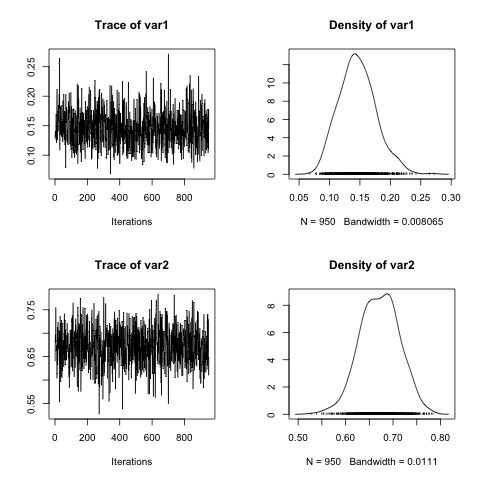
\includegraphics[scale=0.33]{images/metro_5000_100.jpg}
  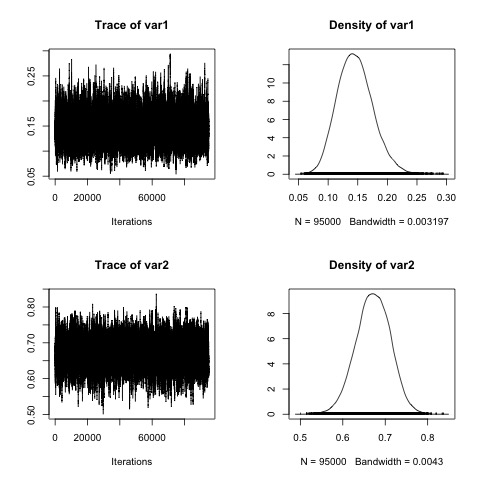
\includegraphics[scale=0.33]{images/metropolis_5000_0.jpg}
  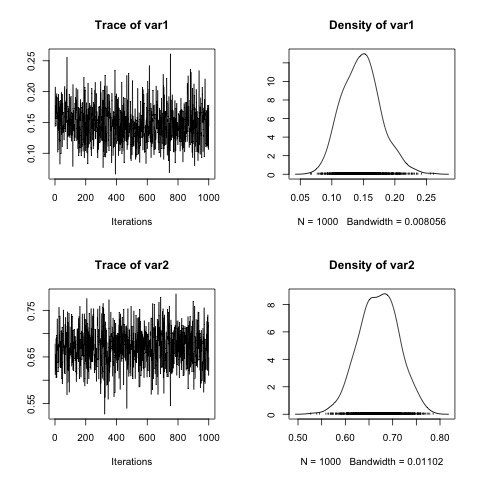
\includegraphics[scale=0.33]{images/metropolis_0_100.jpg}
  \caption{Metropolis Chain Values and Density of Parameters}
  % \label{fig:birds}
\end{figure}

\begin{figure}[h!]
  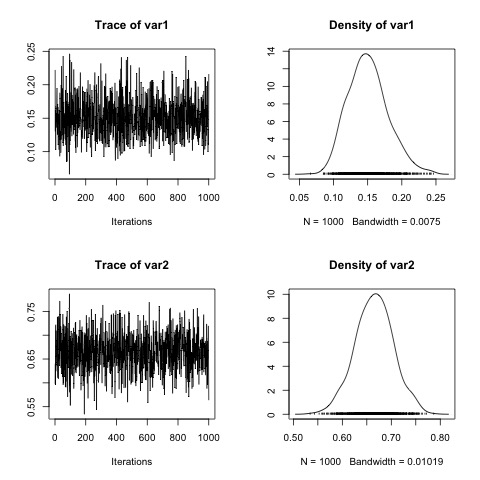
\includegraphics[scale=0.33]{images/gibbs_100_0.jpg}
  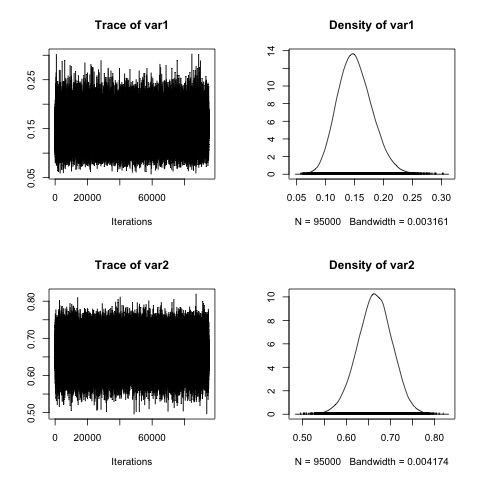
\includegraphics[scale=0.33]{images/gibbs_5000_0.jpg}
  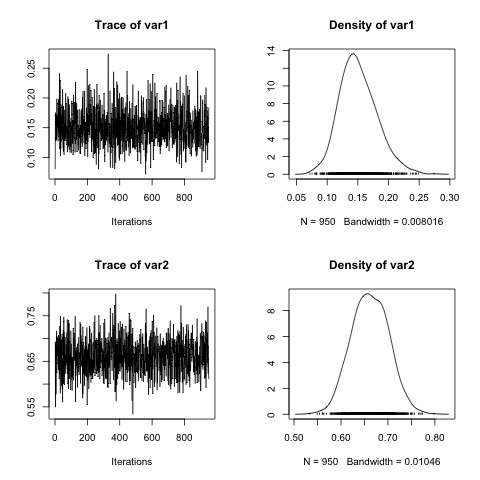
\includegraphics[scale=0.33]{images/gibbs_5000_100.jpg}
  \caption{Gibbs Chain Values and Density of Parameters}
  % \label{fig:birds}
\end{figure}

\begin{figure}[h!]
  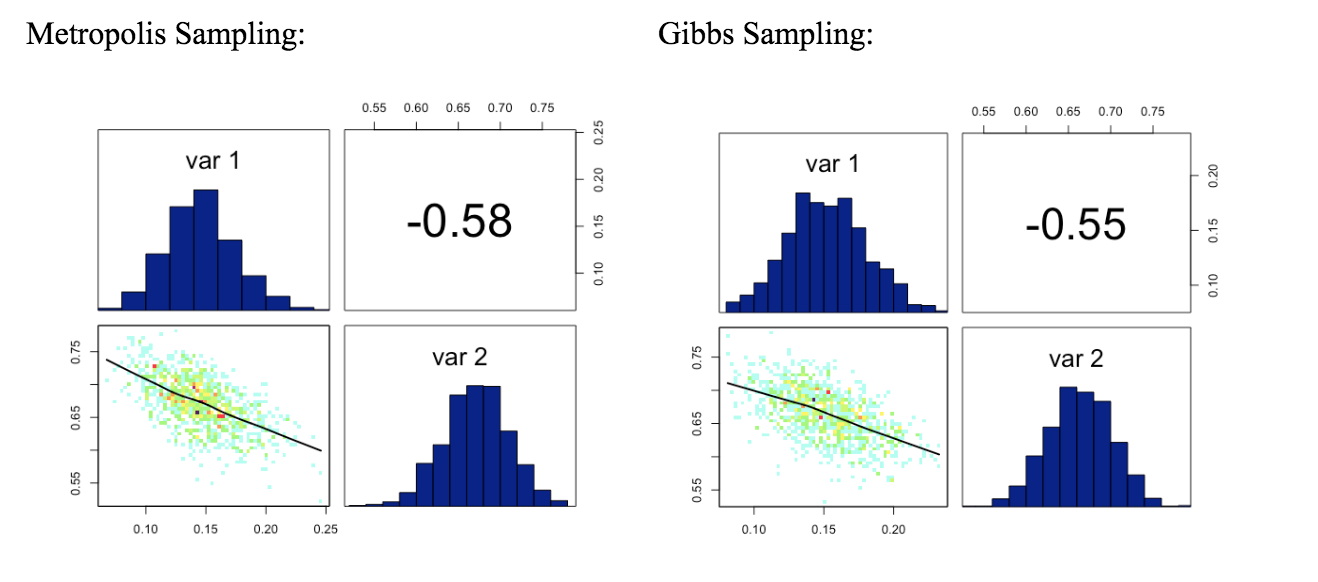
\includegraphics[scale=0.8]{images/correlation.png}
  \caption{Partial Correlations}
  % \label{fig:birds}
\end{figure}

\newpage
\begin{lstlisting}
library(MASS)
library(coda)
library(MCMCpack)
library(BayesianTools)

set.seed(54321)

true_theta<-c(0.1,0.7,0.2)
alpha<-c(2,2,2)
x<-rmultinom(20,size=7,prob = true_theta)   # FIX THIS

gibbs_func<-function(start_value,burnin,thin,iter){
  update<-start_value
  theta_mat<-mat.or.vec(2,iter)
  for(i in 1:iter){
    theta1<-(1-update[2])*(rbeta(1,shape1 = alpha[1]+sum(x[1,]),shape2 = alpha[3]+sum(x[3,])))
    theta2<-(1-theta1)*(rbeta(1,shape1 = alpha[2]+sum(x[2,]),shape2 = alpha[3]+sum(x[3,])))
    update<-c(theta1,theta2)
    theta_mat[,i]<-update
  }
  sample1<-theta_mat[1,][seq(burnin+1,iter,thin)]
  sample2<-theta_mat[2,][seq(burnin+1,iter,thin)]
  
  chain<-matrix(nrow=length(sample1), ncol=2)
  chain[,1]<-sample1
  chain[,2]<-sample2
  
  return(chain)
}

# Posterior
posterior_func <- function(param){
  single_likelihood <- apply(x, 2, function(t) dmultinom(t, prob=param))
  single_prior <- ddirichlet(param, alpha)
  nlikelihood <- sum(log(single_likelihood))
  nprior <- sum(log(single_prior))
  return(nlikelihood + nprior)
  #posterior = sum(apply(post_alpha, 2, function(t) ddirichlet(param, t)))
  # posterior = ddirichlet(param, post_alpha)
}

# Proposal
scale_factor = 1000  # Scale variance of proposal function
proposal_func <- function(param, scale_factor){
  param <- rdirichlet(1, param * scale_factor)
  return(param)
}

# Metropolis MCMC algorithm
run_metropolis_MCMC <- function(start_value, burnin, thin, iter, s = scale_factor){
  theta_mat = array(dim = c(iter+1,3))
  theta_mat[1,1:3] = start_value
  for(i in 1:iter){
    proposal = proposal_func(theta_mat[i,1:3], s)
    prob = exp(posterior_func(proposal) - posterior_func(theta_mat[i,1:3]))
    if (runif(1) < prob){
      theta_mat[i+1,1:3] = proposal
    }else{
      theta_mat[i+1,1:3] = theta_mat[i,1:3]
    }
    
  }
  sample1<-theta_mat[,1][seq(burnin+1,iter,thin)]
  sample2<-theta_mat[,2][seq(burnin+1,iter,thin)] 
  chain<-matrix(nrow=length(sample1), ncol=2)
  chain[,1]<-sample1
  chain[,2]<-sample2
  
  return(chain) 
}

start_value = apply(x, 1, sum) / 140

start = Sys.time()
gibbs_chain<-gibbs_func(start_value[1:2],1000,100,100000)
cat('gibbs time spent: ', Sys.time() - start, '\n')

start = Sys.time()
metro_chain = run_metropolis_MCMC(start_value, 1000,100,100000)
cat("metropolis time spent: ", Sys.time() - start, '\n')
# analysis
summary(gibbs_chain)
par(mar=c(2,2,2,2))
plot(mcmc(gibbs_chain))
plot(mcmc(metro_chain))
# # check partial correlatation btw parameters
combinedchains = mcmc.list(mcmc(gibbs_chain), mcmc(metro_chain))
plot(combinedchains)
gelman.diag(combinedchains)
gelman.plot(combinedchains)
\end{lstlisting}

\end{document}
